\chapter{Economic aspect of Operating Systems }
\label{chap:Economic_aspekt_of_Operating_Systems}


\section{Introduction}

In this section the relevance of Operating Systems in our Economic will be discussed. The importance of Operating Systems in our daily life is not always obvious.
The Operating System is the most important software on a computer. It manages the computer's memory, processes, and all of its software and hardware. 
With the rising amount Digitlization, the Operating System is also becoming more important than ever.

To get an over view on what an Operating System is, please refer to Chapter \ref{sec:WhatIsAnOs}.


\section{Operating System market share}

The Operating System Market is dominated by 4 major players. Android, Microsof Windows, Linux and MacOS.
The market share if the Operting Systems is shown in Figure \ref{fig:Operating_Systems_Market_Share}. 

In the last years, the market share of Android has been increasing. This is due to the rising amount of smartphones and tablets.
Microsoft Windows is still the most used Operating System on Desktops and Laptops.

\begin{figure}[H]
    \centering
    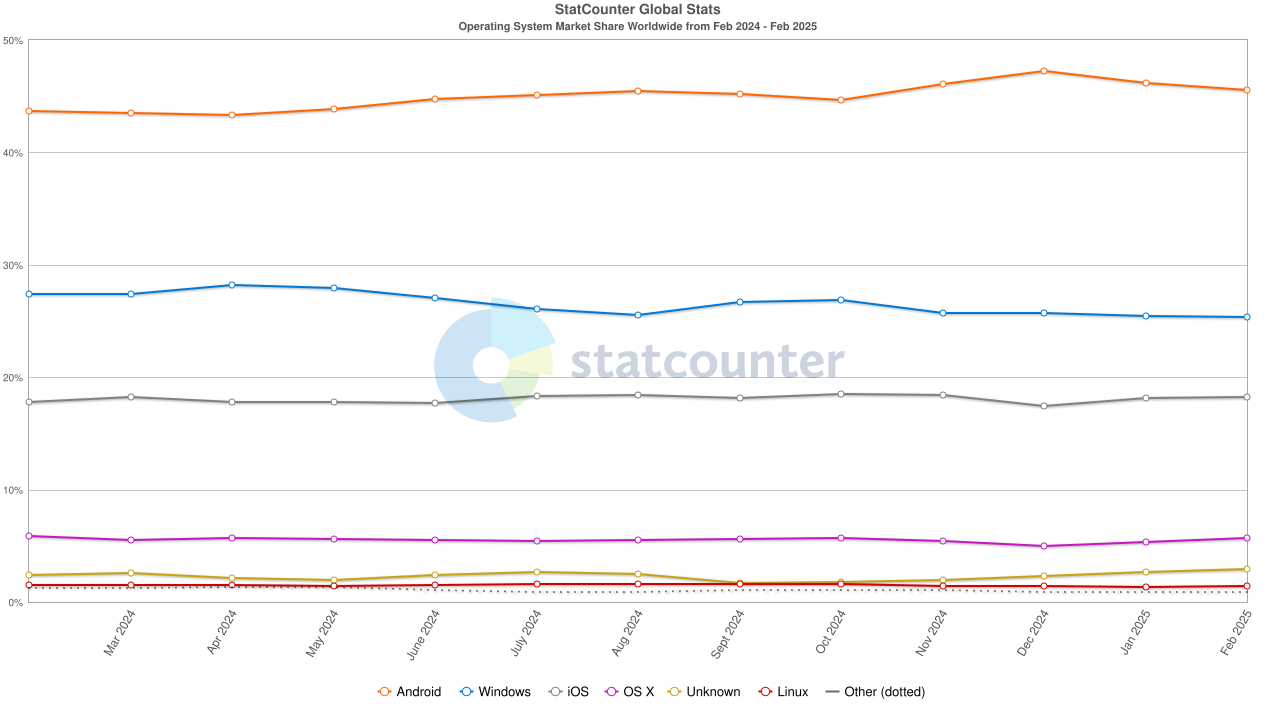
\includegraphics[width=0.8\textwidth]{images/StatCounter-os_combined-ww-monthly-202402-202502.png}
    \caption{Operating Systems Market Share}
    \label{fig:Operating_Systems_Market_Share}
\end{figure}
\cite{OsMarketShare2}

The global market of Operating Systems is expected to reach \textdollar 48,18 billion at a CAGR of 1,9\% in 2026. 
\cite{OsMarketShare3}



\cite{OsMarketShare}
\cite{OsWikipedia}
\author{Florian Prandstetter}